\texttt{OpenNN} has been designed for portability. This means that the library can be built on any operating system with little effort. 
For Windows, project files of Visual C++ are also included.
Regarding Linux, simple makefiles are included in the distribution. 
There should be no problem in building \texttt{OpenNN} on other operating systems, 
since it has been written in ANSI C++.

\subsection*{Windows}

Compiling \texttt{OpenNN} on Windows is easy. 
The library comes with project files for the latest version of Microsoft Visual C++ Express Edition.
When working with another compiler is needed, a project for it must be created.

Microsoft Visual C++ 2010 Express Edition is a free, lightweight,
easy-to-use, and easy-to-learn tools for the hobbyist, novice, and
student developer. It can be downloaded at

\begin{flushleft}
\href{http://www.microsoft.com/express}{http://www.microsoft.com/express}
\end{flushleft}

\texttt{OpenNN} includes the \lstinline"opennn.sln" solution file for that
compiler in the \lstinline"build/visual_studio" folder.

To open the \texttt{OpenNN} project just double click on that file. A
similar window than that depicted in Figure
\ref{VisualStudioSolution} should come up.

\begin{figure}[h!]
\begin{center}
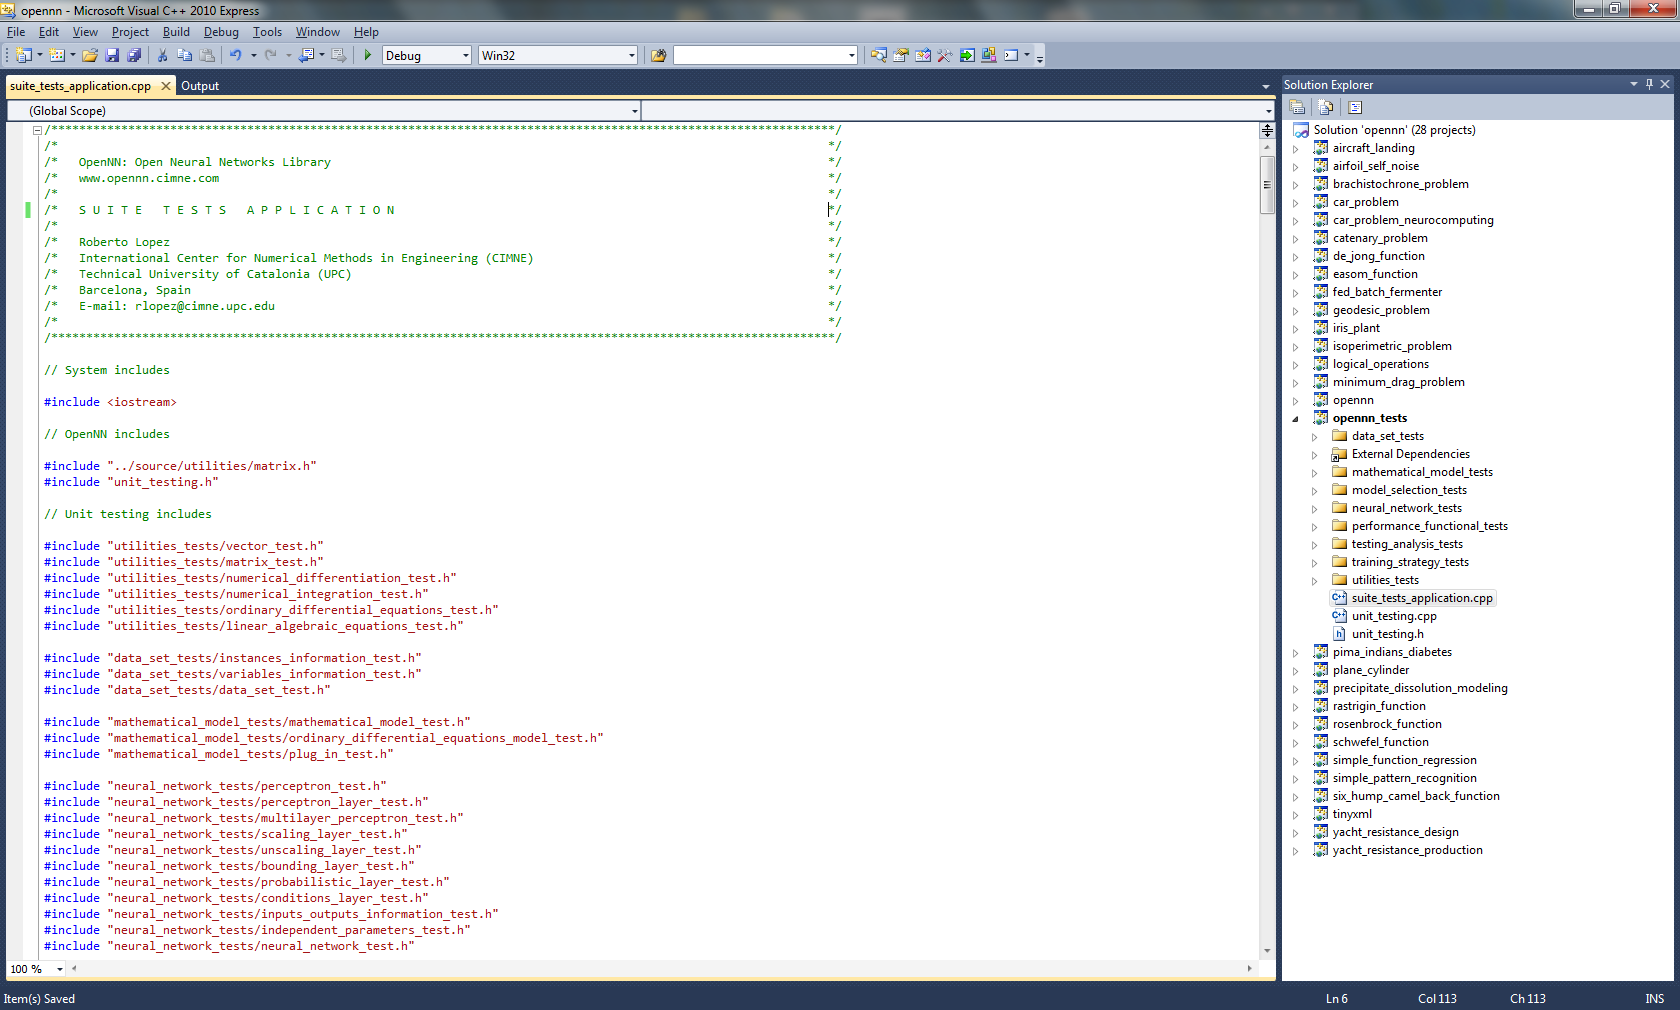
\includegraphics[width=1.0\textwidth]{preliminaries/visual_studio}
\caption{Microsoft Visual C++ 2010 solution view.}\label{VisualStudioSolution}
\end{center}
\end{figure}

Pressing \lstinline"Ctrl+F5" will compile, build and run the
test suite application. A MS-DOS console should appear with the following message:

\begin{lstlisting}
...

OpenNN test suite results:
Tests run: tests_run
Tests passed: tests_run
Tests failed: 0
Test OK
\end{lstlisting}

This guarantees that \texttt{OpenNN} has been compiled properly, toguether with all the libraries included.
On the other hand, many practical applications can be found in the same solution. 

Note that project files of other versions than Visual C++ 2010 Express Edition are
not guaranteed to be opened. In that case, and in order to use \texttt{OpenNN}, a new solution should be
created. 


\subsection*{Linux}

Compilation of OpenNN in Linux is straight-forward, since simple makefiles are here provided.
In order to do that, the following steps must be performed:

\subsubsection*{1. Extract the \lstinline"OpenNN.zip" file to the installation
folder.}

To install \texttt{OpenNN} from the download location
\lstinline"DOWNLOAD_DIRECTORY" into the installation location
\lstinline"INSTALLATION_DIRECTORY" use the following commands:

\begin{lstlisting}
>cd DOWNLOAD_DIRECTORY
>unzip OpenNN.zip INSTALLATION_DIRECTORY
\end{lstlisting}

You can specify any name for the installation folder. The name
\lstinline"OpenNN" will be used here. 

\subsubsection*{2. Run the test suite makefile.}

The folder \lstinline"\OpenNN\build\make" contains a 
makefile for a test suite of the whole library.
To run that makefile type the following commands on
the terminal:

\begin{lstlisting}
>cd \OpenNN\build
>make -f opennn_tests_makefile
\end{lstlisting}

This compiles all the classes included in \texttt{OpenNN} and builds a test suite for them.
To verify the installation, run the test suite executable:

\begin{lstlisting}
>./opennn_tests
\end{lstlisting}

If nothing has been wrong, the following message should appear on
the terminal:

\begin{lstlisting}
...
OpenNN test suite results:
Tests run: tests_run
Tests passed: tests_run
Tests failed: 0
Test OK
\end{lstlisting}

\subsubsection*{3. Run an example makefile.}

The folder \lstinline"\OpenNN\build" also contains  
makefiles for all the examples included in the distribution. 
To run the simple function regression example, type the following commands on
the terminal:

\begin{lstlisting}
>cd \OpenNN\build\make
>make -f simple_function_regression_makefile 
\end{lstlisting}

Once all the classes have been compiled and the application has been built, 
you can run the example:

\begin{lstlisting}
>./simple_function_regression
\end{lstlisting}

Read the application code to see what the simple function regression example does. 

\subsubsection*{4. Removing a OpenNN Installation}

To remove an \texttt{OpenNN} installation, enter the following command on the terminal:

\begin{lstlisting}
>rm -rf \$OpenNN
\end{lstlisting}

This will delete the whole \texttt{OpenNN} folder.
